\documentclass[sigconf, nonacm]{acmart}

% should be fine as it is
\newcommand\vldbauthors{\authors}
\newcommand\vldbtitle{\shorttitle} 
% leave empty if no availability url should be set
\newcommand\vldbavailabilityurl{https://github.com/cs4248-nlp-gec/typo-gec}
% whether page numbers should be shown or not, use 'plain' for review versions, 'empty' for camera ready
\newcommand\vldbpagestyle{plain} 

\begin{document}
\title{Enhancing Transformer-Based Grammatical Error Correction with Contextual Typo Adaptation for Noisy Text Environments}

%%
%% The "author" command and its associated commands are used to define the authors and their affiliations.
\author{Lee Zong Xun}
\affiliation{%
  \institution{National University of Singapore}
}
\email{lzongxun@u.nus.edu}

\author{Lee Zong Xun}
\affiliation{%
  \institution{National University of Singapore}
}
\email{lzongxun@u.nus.edu}

\author{Lee Zong Xun}
\affiliation{%
  \institution{National University of Singapore}
}
\email{lzongxun@u.nus.edu}

\author{Lee Zong Xun}
\affiliation{%
  \institution{National University of Singapore}
}
\email{lzongxun@u.nus.edu}

\author{Lee Zong Xun}
\affiliation{%
  \institution{National University of Singapore}
}
\email{lzongxun@u.nus.edu}

\author{Lee Zong Xun}
\affiliation{%
  \institution{National University of Singapore}
}
\email{lzongxun@u.nus.edu}

\begin{abstract}
Text correction systems (e.g., spell checkers) have been used to improve the quality of computerized text by detecting and correcting errors. In this project, we investigated usage of GECToR's capabilities, predominantly used for correcting grammatical errors in texts that are well-composed and polished, for use in "noisy" textual environments rife with less structured language. We have found that GECToR is insufficiently robust for correcting spelling errors and word variances, particularly, suffering from overcorrections (text rewrites). Thus, we proposed a neural-based text corrector with a two-stage structure to alleviate issues of overcorrections while exploiting the benefits of a neural corrector. Our method consists of a rule-based error detector and an attention neural error corrector with contextual attention.  This novel architecture allows GECToR to produce corrections based on both the erroneous text and its context without the need for an end-to-end structure. 

% This project seeks to assess and improve the GECToR model capabilities, predominantly used for correcting grammatical errors in texts that are well-composed and polished, for use in "noisy" textual environments rife with less structured language. We intend to complement the model with a context-aware typo correction model, thereby fully leveraging the power of transformers to optimize its efficacy in both typo rectification and grammatical error resolution.
\end{abstract}
\maketitle % important, do not remove
%%% VLDB block start %%%
\ifdefempty{\vldbavailabilityurl}{}{
\begingroup\small\noindent\raggedright\textbf{Artifact Availability:}
The source code, data, and/or other artifacts have been made available at \url{\vldbavailabilityurl}.
\endgroup
}
%%% VLDB block end %%%

\section{Introduction}

Grammar error correction (GEC) is one of the most prominent tasks in natural language processing, with numerous transformer-based models [insert references to other models] gaining prominence in recent years. Of particular interest is the tagging-based GECToR model, developed by [insert names and reference here] (https://aclanthology.org/2020.bea-1.16.pdf), which obtained State-Of-The-Art (SOTA) performance when tested against the CoNLL-2014 and BEA-2019 datasets. One shortcoming, however, is its capacity to handle spelling errors, otherwise colloquially referred to as typos. While preliminary observations found a decent capacity to handle basic spelling errors, it was generally unable to handle more complex typos (A more thorough analysis is provided in Section [insert section here]). We attribute this shortcoming primarily due to the scale of GECToR model itself: intuitively, we do not expect a model, trained primarily on the more general task of grammar correction, to be similarly capable on the more specific task of spelling correction. The focus of the paper, therefore, is to develop and refine GECToR to effectively handle and accurately correct typos and semantic errors commonly found in "noisy" digital text environments, while respecting and preserving the unique communicative styles and intentions of users. 

To this end, we employ a 2-phase approach: The first model or phase is designed to parse and pinpoint typographical errors or other similar mistakes that tend to occur in digital communication. Once these initial errors are detected and fixed, the corrected sentence is then passed to the second phase or model, which focuses on more complex grammatical corrections. This step ensures that grammar is checked in a relatively clean text, possibly reducing the complexity of this task. We explore and compare the effectiveness of 3 different types of spelling correction models in the first phase: a naive, edit-distance based model proposed by Norvig (https://norvig.com/spell-correct.html), a statistical-based n-grams model, and a transformer-based sequence-to-sequence model. GeCToR is primarily employed for the second-phase model, with further comparisons done using pre-trained and re-trained versions of the model. 

\section{Preliminaries}

\begin{figure*}
    \centering
    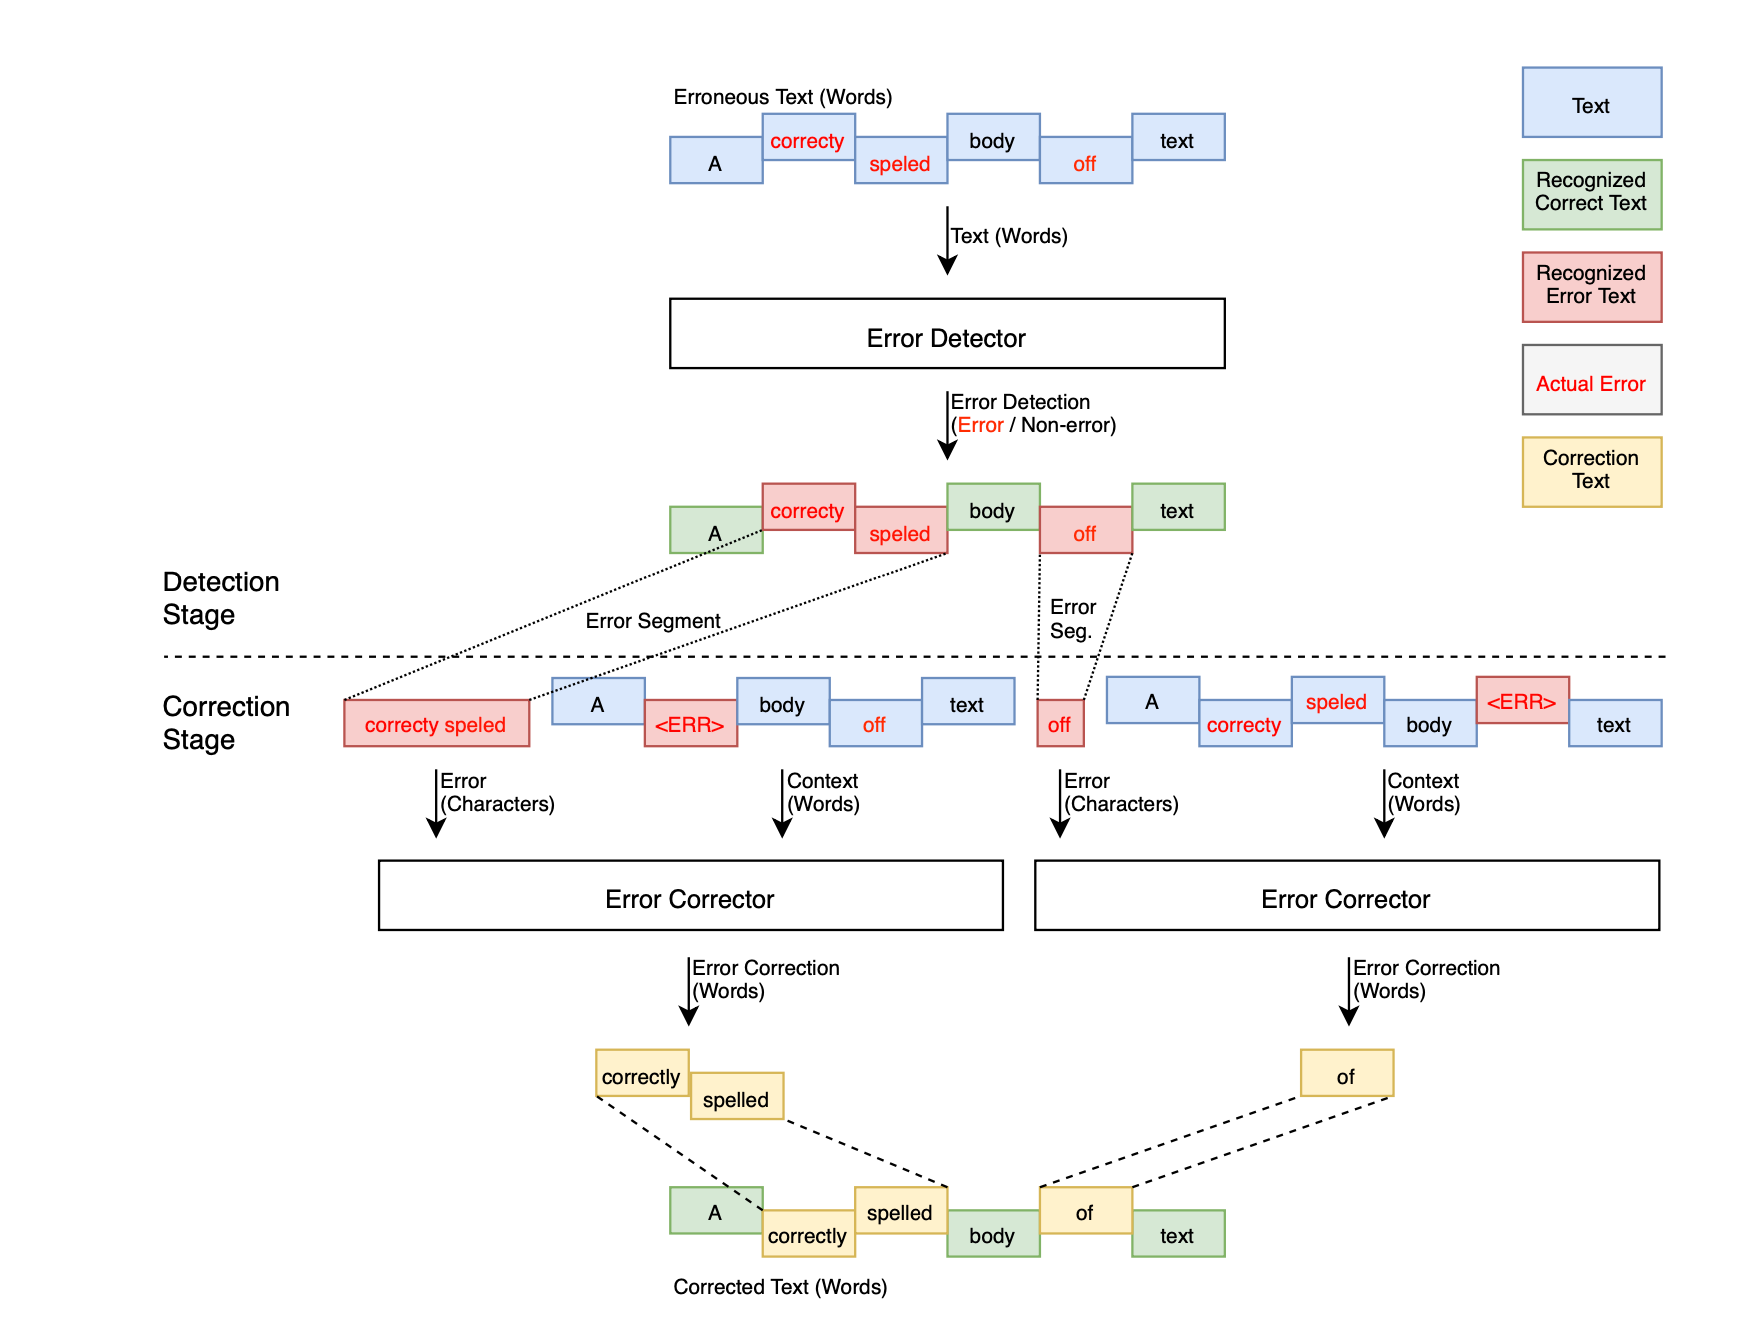
\includegraphics[width=1\linewidth]{figures/overview}
    \caption{Overview of textual correction system}
    \label{fig:enter-label}
\end{figure*}

\subsection{Data Augmentation}

We experimented with injecting noise into the dataset during model pretraining to help increase the number of erroneous examples in the training set. Our method was inspired by the data augmentation technique employed in the copy- augmented transformer [12]. However, we inject character errors rather than word errors. We inject three types of errors:
a random character deletion, a random character substitu- tion, and a random character insertion. Each type of error possesses a 3\% probability of appearing for every position in the text. When a character is replaced or inserted, the replacement character is chosen at random based on the distribution of that character in the training set.

\subsection{An overview of GECToR}

Here's an example of how to reference \autoref{fig:duck}.

\begin{figure}
  \centering
  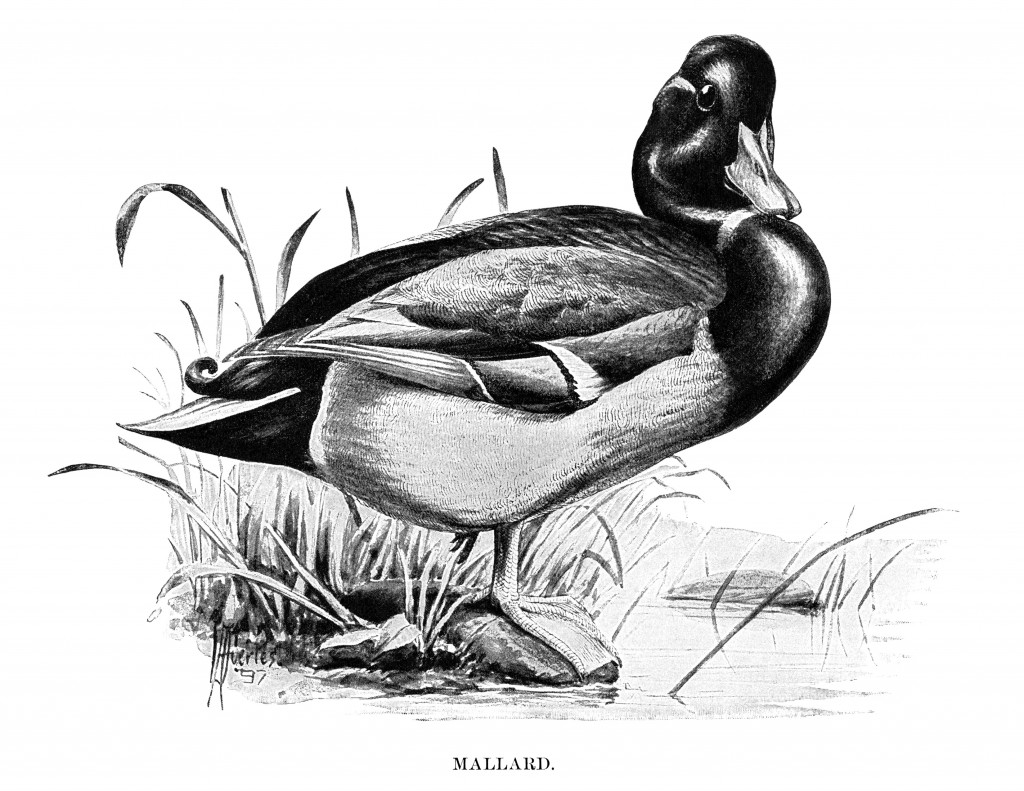
\includegraphics[width=\linewidth]{figures/duck}
  \caption{Quack quack}
  \label{fig:duck}
\end{figure}

\subsection{Spelling Correction Models}

Curabitur vitae nulla dapibus, ornare dolor in, efficitur enim. Cras fermentum facilisis elit vitae egestas. Nam vulputate est non tellus efficitur pharetra. Vestibulum ligula est, varius in suscipit vel, porttitor id massa. Cras facilisis suscipit orci, ac tincidunt erat.

\subsection{Synthetic Corpus Generation}

Curabitur vitae nulla dapibus, ornare dolor in, efficitur enim. Cras fermentum facilisis elit vitae egestas. Nam vulputate est non tellus efficitur pharetra. Vestibulum ligula est, varius in suscipit vel, porttitor id massa. Cras facilisis suscipit orci, ac tincidunt erat.

\section{Related Words}
Curabitur vitae nulla dapibus, ornare dolor in, efficitur enim. Cras fermentum facilisis elit vitae egestas. Nam vulputate est non tellus efficitur pharetra. Vestibulum ligula est, varius in suscipit vel, porttitor id massa. Cras facilisis suscipit orci, ac tincidunt erat.

\section{Experiments}
Curabitur vitae nulla dapibus, ornare dolor in, efficitur enim. Cras fermentum facilisis elit vitae egestas. Nam vulputate est non tellus efficitur pharetra. Vestibulum ligula est, varius in suscipit vel, porttitor id massa. Cras facilisis suscipit orci, ac tincidunt erat.

\section{Discussion}

Curabitur vitae nulla dapibus, ornare dolor in, efficitur enim. Cras fermentum facilisis elit vitae egestas. Nam vulputate est non tellus efficitur pharetra. Vestibulum ligula est, varius in suscipit vel, porttitor id massa. Cras facilisis suscipit orci, ac tincidunt erat.

\section{Conclusion}

Curabitur vitae nulla dapibus, ornare dolor in, efficitur enim. Cras fermentum facilisis elit vitae egestas. Nam vulputate est non tellus efficitur pharetra. Vestibulum ligula est, varius in suscipit vel, porttitor id massa. Cras facilisis suscipit orci, ac tincidunt erat.

\begin{table*}[t]
  \caption{A double column table.}
  \label{tab:commands}
  \begin{tabular}{ccl}
    \toprule
    A Wide Command Column & A Random Number & Comments\\
    \midrule
    \verb|\tabular| & 100& The content of a table \\
    \verb|\table|  & 300 & For floating tables within a single column\\
    \verb|\table*| & 400 & For wider floating tables that span two columns\\
    \bottomrule
  \end{tabular}
\end{table*}

\section{References}

Curabitur vitae nulla dapibus, ornare dolor in, efficitur enim. Cras fermentum facilisis elit vitae egestas. Nam vulputate est non tellus efficitur pharetra. Vestibulum ligula est, varius in suscipit vel, porttitor id massa. Cras facilisis suscipit orci, ac tincidunt erat.


% Examples of table references 
\autoref{tab:commands} \autoref{tab:freq} 

\begin{table}[hb] % h asks to places the floating element [h]ere.
  \caption{Frequency of Special Characters}
  \label{tab:freq}
  \begin{tabular}{ccl}
    \toprule
    Non-English or Math & Frequency & Comments\\
    \midrule
    \O & 1 in 1000& For Swedish names\\
    $\pi$ & 1 in 5 & Common in math\\
    \$ & 4 in 5 & Used in business\\
    $\Psi^2_1$ & 1 in 40\,000 & Unexplained usage\\
  \bottomrule
\end{tabular}
\end{table}

% \begin{displaymath}
%   \sum_{i=0}^{\infty} x + 1
% \end{displaymath}

% \begin{equation}
%   \sum_{i=0}^{\infty}x_i=\int_{0}^{\pi+2} f
% \end{equation}

Curabitur vitae nulla dapibus, ornare dolor in, efficitur enim. Cras fermentum facilisis elit vitae egestas. Nam vulputate est non tellus efficitur pharetra. Vestibulum ligula est, varius in suscipit vel, porttitor id massa. Cras facilisis suscipit orci, ac tincidunt erat.

\section{Citations}

Some examples of references. A paginated journal article~\cite{Abril07}, an enumerated journal article~\cite{Cohen07}, a reference to an entire issue~\cite{JCohen96}, a monograph (whole book) ~\cite{Kosiur01}, a monograph/whole book in a series (see 2a in spec. document)~\cite{Harel79}, a divisible-book such as an anthology or compilation~\cite{Editor00} followed by the same example, however we only output the series if the volume number is given~\cite{Editor00a} (so Editor00a's series should NOT be present since it has no vol. no.), a chapter in a divisible book~\cite{Spector90}, a chapter in a divisible book in a series~\cite{Douglass98}, a multi-volume work as book~\cite{Knuth97}, an article in a proceedings (of a conference, symposium, workshop for example) (paginated proceedings article)~\cite{Andler79}, a proceedings article with all possible elements~\cite{Smith10}, an example of an enumerated proceedings article~\cite{VanGundy07}, an informally published work~\cite{Harel78}, a doctoral dissertation~\cite{Clarkson85}, a master's thesis~\cite{anisi03}, an finally two online documents or world wide web resources~\cite{Thornburg01, Ablamowicz07}.

\begin{acks}
 This work was supported by the [...] Research Fund of [...] (Number [...]). Additional funding was provided by [...] and [...]. We also thank [...] for contributing [...].
\end{acks}

%\clearpage

\bibliographystyle{ACM-Reference-Format}
\bibliography{sample}

\end{document}
